% !TEX root = ../../report.tex

\section{Описание ролей}

Исходя из анализа предметной области и требований к системе, выделены следующие роли пользователей:

\begin{enumerate}
    \item гость (неавторизованный пользователь);
    \item покупатель;
    \item продавец;
    \item администратор;
    \item аналитик.
\end{enumerate}

\textbf{Гость} --- неавторизованный пользователь, обладающий правами на просмотр каталога товаров, карточки товара (включая информацию о товаре, историю изменения цены и отзывы), а также на прохождение процедуры авторизации (регистрации или входа в систему).

\textbf{Покупатель} --- авторизованный пользователь, который, помимо возможностей гостя, может оформлять заказы (добавлять товары в корзину, выбирать адрес доставки, производить оплату) и оставлять отзывы на приобретённые товары. Каждый покупатель управляет собственными адресами доставки. Один покупатель может оставить не более одного отзыва на конкретный товар.

\textbf{Продавец} --- авторизованный пользователь, зарегистрировавший профиль компании. Продавец управляет собственными товарами (добавление, редактирование, удаление), просматривает входящие заказы и фиксирует их переходы по статусам отгрузки и доставки. Также продавцу доступна статистика продаж за указанный период.

\textbf{Администратор} --- пользователь с функциями модератора платформы. Наследует возможности гостя (просмотр каталога, карточки товара, авторизация). Администратор управляет категориями товаров (создание, редактирование, удаление), может удалять пользователей, продавцов, товары и отзывы. Также ему доступен просмотр всех заказов в системе, отчётов и статистики продаж. Администратор не создаёт товары, не оформляет заказы и не оставляет отзывы.

\textbf{Аналитик} --- пользователь, обладающий правами на чтение всех данных системы без возможности их модификации. Роль предназначена для формирования отчётов: топ товаров по продажам, динамика заказов по времени, распределение продаж по категориям.

Отдельная роль для управления складскими остатками не выделяется. Количество товара относится к данным товара, которыми управляет продавец, а резерв изменяется при обработке заказов.

Диаграмма вариантов использования приведена на рисунке~\ref{fig:usecase}.

\begin{figure}[H]
    \centering
    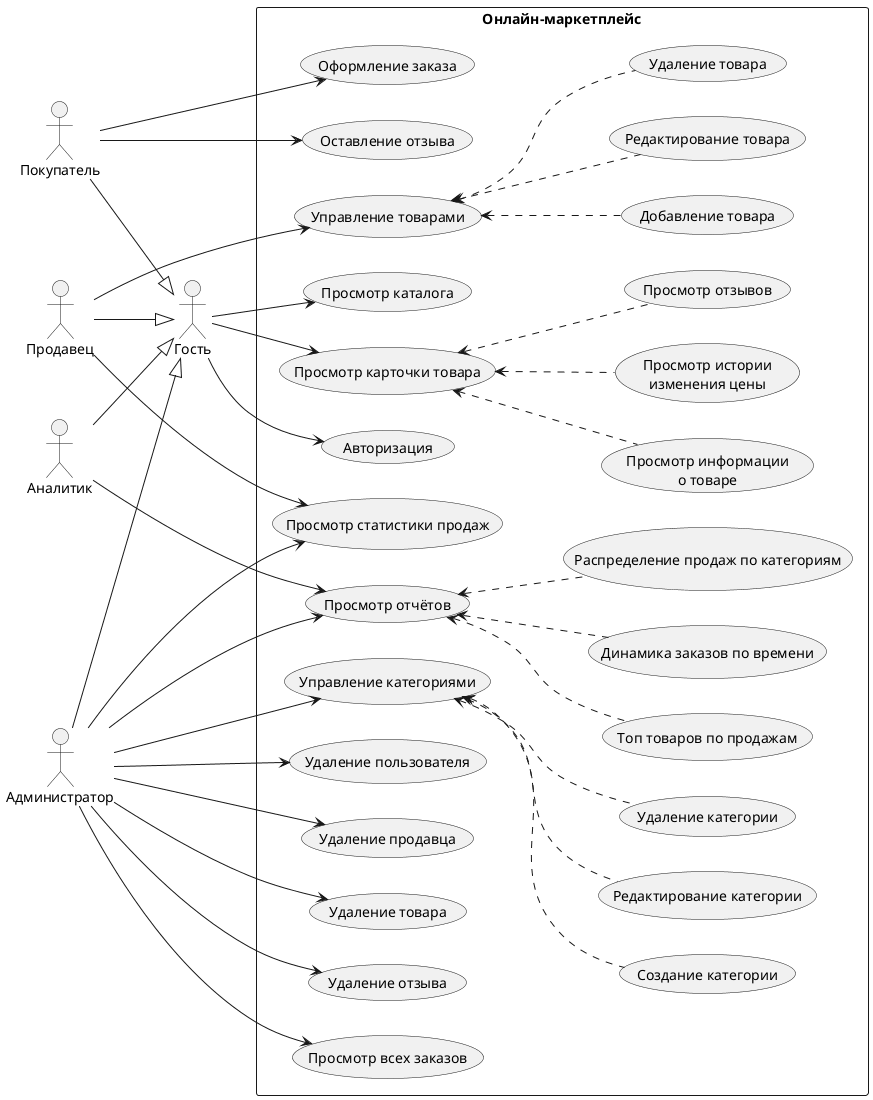
\includegraphics[width=\textwidth]{img/UseCases.png}
    \caption{Диаграмма вариантов использования}
    \label{fig:usecase}
\end{figure}

Каждая авторизованная роль наследует возможности гостя. Администратор, в отличие от покупателя и продавца, не наследует их бизнес-действий, а обладает собственным набором операций, ориентированных на модерацию и контроль данных платформы.
